\documentclass{beamer}   %, handout

\usepackage{graphicx}

%\usetheme{Szeged}
%\usecolortheme{dolphin}

%\setbeamertemplate{navigation symbols}{}

\setcounter{equation}{0}

%%%%%%%%%%%%%%%%%%%%%%%%%%%%%%%%%
%%%%%%  USE Latex => pdf !!!!!!!!
%%%%%%%%%%%%%%%%%%%%%%%%%%%%%%%%%

\title{Reduction Loop Example}
%% Which is to say types as they are used in practice in software development and as represented in theory in categories and in syntactic type theories.
%% There is also a subplot concerning representation of context which certain types depend on -- again represented in practice and in theory. 
\author{John Cartmell}
\institute{Ad Otium}
\date{19 June 2020}
\begin{document}

\begin{frame}
\titlepage
\end{frame}

\begin{frame}{Introduction 10}

I am struggling to prove my main theorem and so look for a counter example.
I wrote this on a white board yesterday
\begin{center}
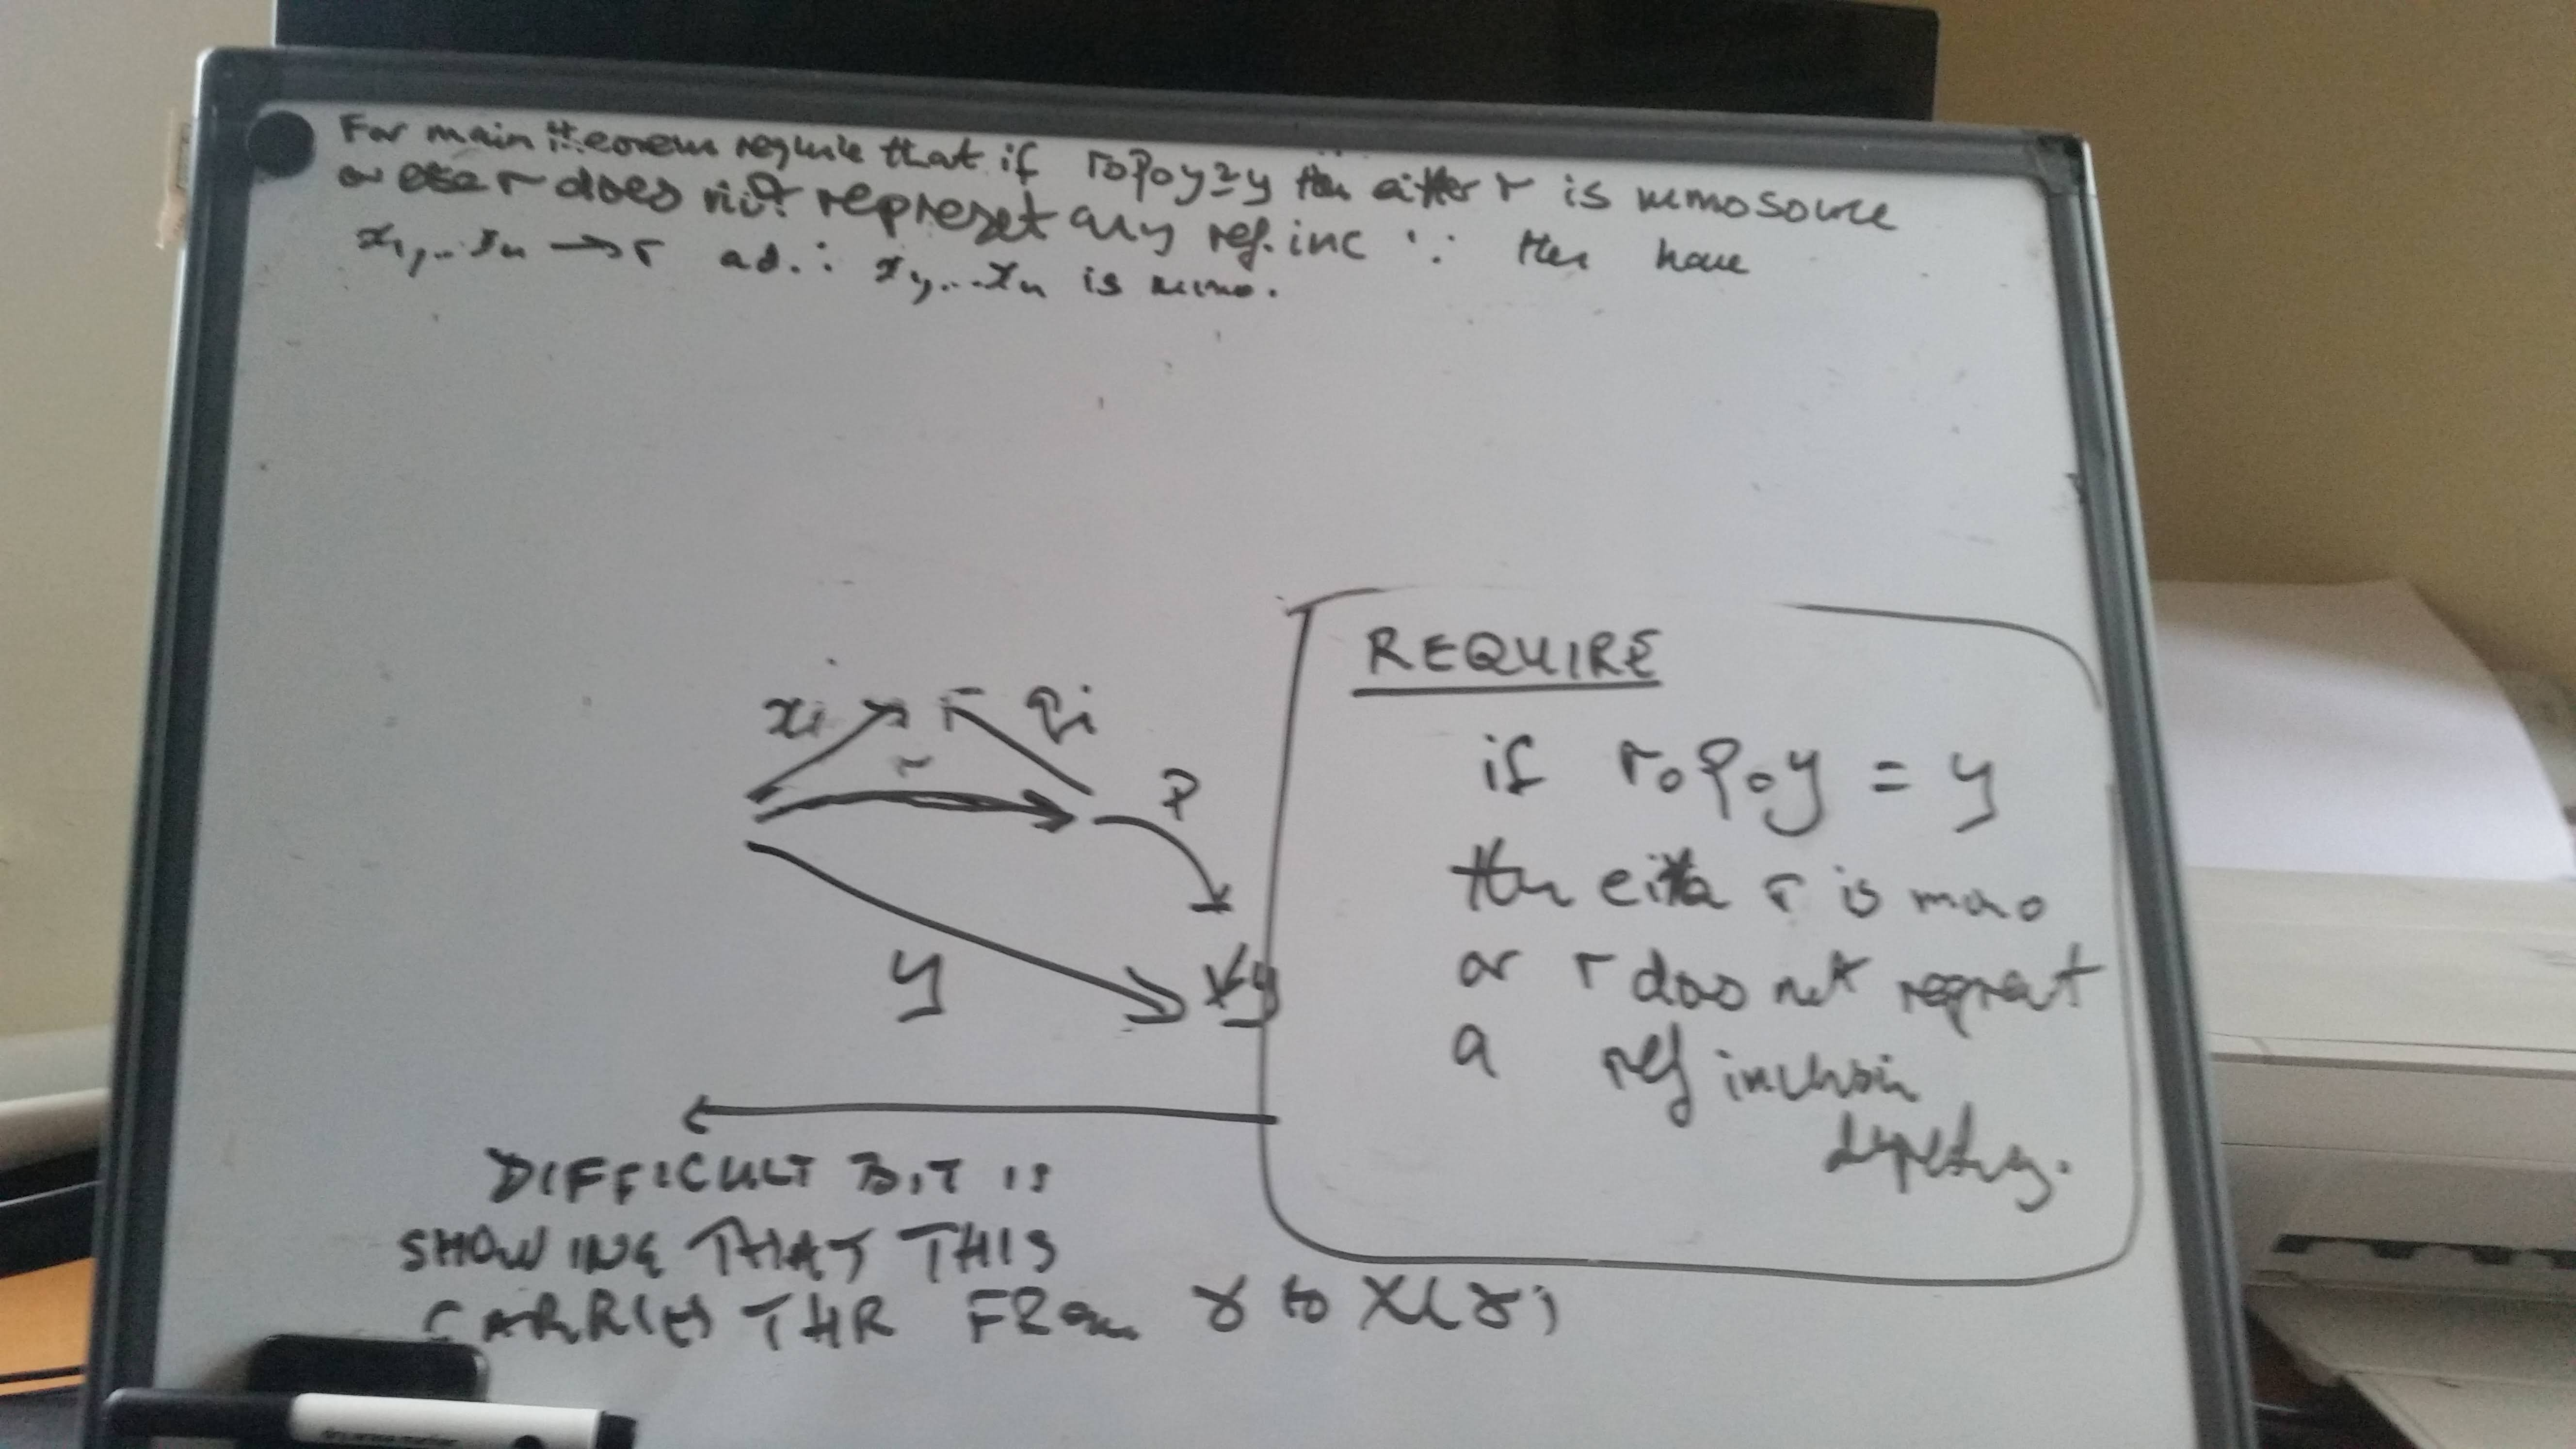
\includegraphics[width=10cm]{20200619_10.jpg}
\end{center}
What follows are my notes from today. 19 June 2020
\end{frame}

\newcommand{\slide}[2][]{\begin{frame}{#2}
\begin{center}
\includegraphics[width=11cm]{20200619_#2.jpg}
\end{center}
#1
\end{frame}}

\slide{20}
%\slide{30}  not helpful
\slide{40}
\slide{50}
\slide{60}
\slide{70}
\slide{80}
\slide[I have a problem - this is the counter example i was looking for]{90}
\slide{100}
\slide[\footnotesize Suppose we reinstate relationship-like clause in definition of well-formulated then we wouldn't have a counterexample because
this model wouldn't be well-formulated. Therefore consider here (a different model) what if $r \circ s$ is relationship-like i.e. if $s$ is identifying-like.]{110}
\slide[How can we fix the original model though? Not be adding x for example]{120}
\slide[\footnotesize We can fix the original model by moving attributes $x_1$ and $x_2$ to entity type $b$. Seems a bit strange because moving to a more general type $b$ from a more specific type $a$.
Just a hint here that further conditions might come along one day to reduce duplication in such $x_i$, $s_i$.]
 {130}


\end{document}